\documentclass{standalone}
\usepackage{tikz}
\usetikzlibrary{arrows.meta}
\tikzset{label/.style = {inner sep=1pt, fill=white}}
%\tikzset{nd/.style={circle, inner sep=0pt}}
\tikzset{nd/.style={inner sep=1pt}}
\tikzset{>=Latex}
\tikzset{arc/.style = {->, semithick, >=Latex}}
\begin{document}
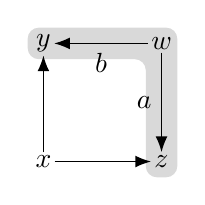
\begin{tikzpicture}

\fill [rounded corners, color=gray!30] (-0.2, 1.7) -- (-.2,1.3) -- (1.3,1.3) -- (1.3,-0.2) -- (1.7,-.2) -- (1.7,1.7) -- cycle;

    \node[nd] (A) at (0,0) {$x$};
    \node[nd] (B) at (0,1.5) {$y$};
    \node[nd] (C) at (1.5,0) {$z$};
    \node[nd] (D) at (1.5,1.5) {$w$};
    \draw[arc] (A) to (B);
    \draw[arc] (D) to node[midway,below] {$b$} (B);
    \draw[arc] (A) to (C);
    \draw[arc] (D) to node[midway,left] {$a$} (C);

    
    %\draw [rounded corners, color = gray, line width = 10pt, opacity = 0.3] (D) to (C) to (D) to (B) to cycle;
\end{tikzpicture}
\end{document}\textbf{}